\documentclass{ximera}
\begin{document}
\title{Setting up the repository}
\begin{enumerate}
\item Create a directory and change to that directory.
In this example, we will create a director called sampleCourse.
\begin{center}
\begin{verbatim}
mkdir sampleCourse&& cd sampleCourse 
\end{verbatim}
\end{center}
\item A Ximera course consists of a directory containing
at least
a text file called \verb!course.xim!. This file contains
at least the name of the course, a description of the course,
and the names of all the activity \LaTeX\ files in the order
they should be presented. In the example below
there is one activity file \verb!example.tex!
written without the extension \verb!.tex!,
which lives in a directory \verb!example!.
\begin{verbatim}
---
name: Getting Started with Ximera
description: This is a Ximera activity explaining how to get started
with Ximera for instructors.
---

example/example
\end{verbatim}
In general, it is a sensible policy to have each
activity in its own directory, of the same name. This facilitates the
sharing of activities between collaborators and makes reusing existing
activities much easier. Later in this course, we will see examples of
how to use existing activities and courses rather than starting from scratch.

\item As mentioned above, we need to add a directory
called \verb!example! containing a file called \verb!example.tex!.
\begin{verbatim}
mkdir example
cd example
touch example.tex
\end{verbatim}

\item The activity in \verb!example.tex!
should be in the documentclass \verb!ximera!
and should contain the title of the activity.
For example,
\begin{verbatim}
\documentclass{ximera}
\begin{document}
\title{Our first activity}
\end{document}
\end{verbatim}
The activity at this stage contains no content.

\item On \verb!github.org! create a repository as shown
in the image below.
\begin{center}
\begin{image}
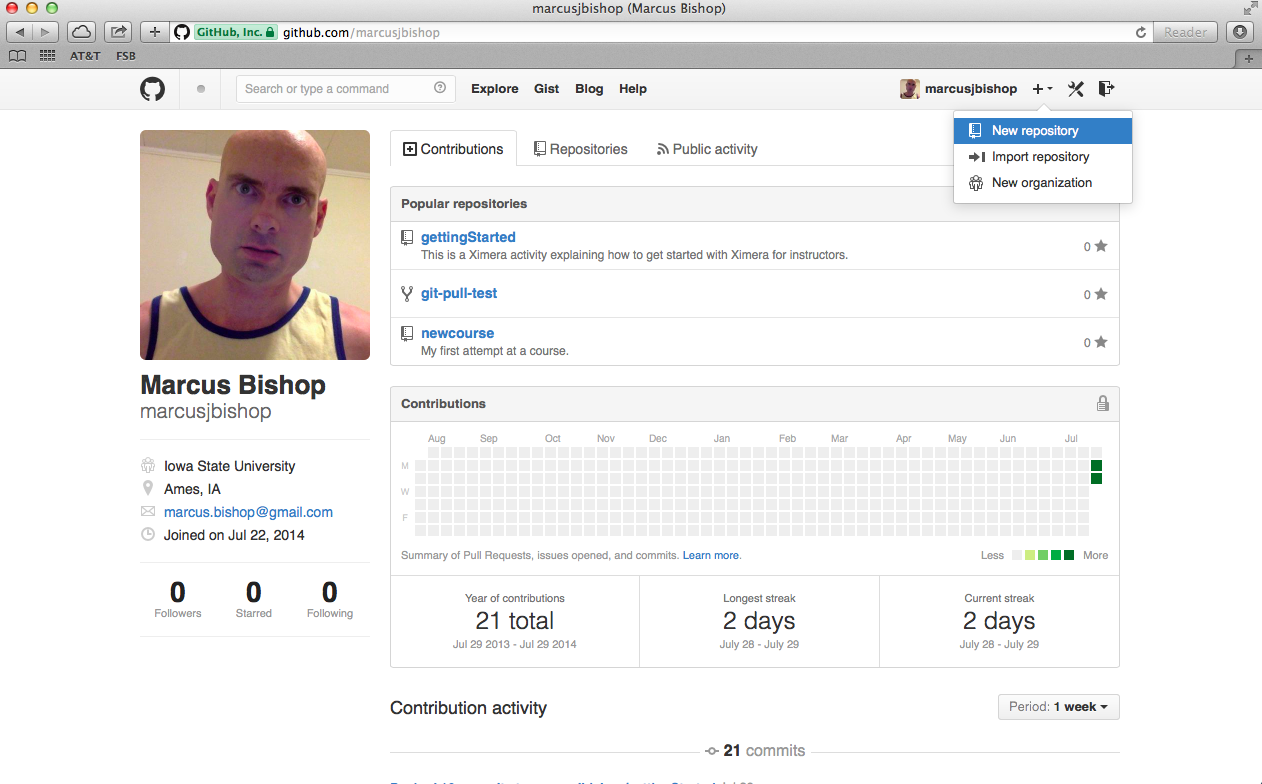
\includegraphics[scale=.3]{RepoInit.png}
\end{image}
\end{center}

\item Follow the instructions in \verb!github! to set up
the repository, accepting all default settings.
This should include some further git commands that
will push your work above to \verb!github!:
\begin{verbatim}
touch README.md
git init
git add README.md
git commit -m "first commit"
git remote add origin https://github.com/marcusjbishop/example.git
git push -u origin master
\end{verbatim}
These commands also appear on \verb!github!.

\item Write something in \verb!README.md!

\item Click on \verb!settings! on the \verb!github! page
for this repository created above,
and then \verb!Webhooks & Services!
\begin{center}
\begin{image}
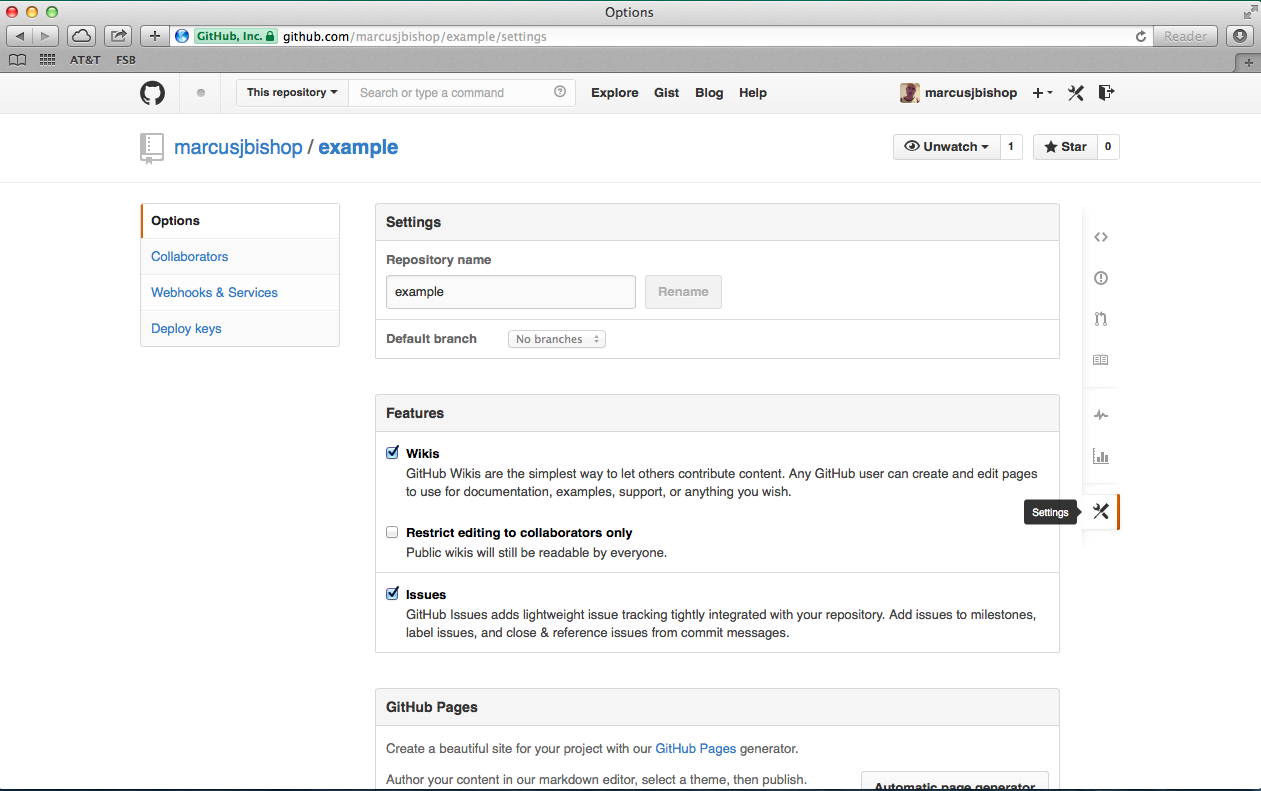
\includegraphics[scale=.3]{Webhook.png}
\end{image}
\end{center}
Now click the \verb!Add webhook! button.
Put \verb!http://ximera.osu.edu/github!
into the \verb!Payload URL! field and
\verb!8mi0tsrje9n3asPu86XC198G1XSdZj!
into the \verb!Secret! field.

\end{enumerate}
\end{document}
